\subsection{Speedy Signals: What Affects Transmission Line Velocity?}

\begin{tcolorbox}[colback=gray!10, colframe=black, title=E9F02]
Which of the following has the biggest effect on the velocity factor of a transmission line?
\begin{enumerate}[label=\Alph*.]
    \item The characteristic impedance
    \item The transmission line length
    \item \textbf{The insulating dielectric material}
    \item The center conductor resistivity
\end{enumerate} \end{tcolorbox}

\subsubsection{Explanation of the Correct Answer}


The velocity factor is given by the equation:

\[
VF = \frac{c}{v} = \frac{1}{\sqrt{\epsilon_r}}
\]

where:
- \( c \) is the speed of light in vacuum (approximately \( 3 \times 10^8 \) m/s),
- \( v \) is the speed of the signal in the transmission line,
- \( \epsilon_r \) is the relative permittivity of the insulating material.

This indicates that the choice of dielectric material impacts the relative permittivity and, consequently, the velocity factor.

\subsubsection{Related Concepts}
To further understand the velocity factor and its determinants, we need to consider:
1. \textbf{Dielectric Materials:}: The differences in molecular structure and bonding among various dielectrics lead to changes in their permittivity, thus affecting the VF.
2. \textbf{Characteristic Impedance:}: While it plays a crucial role in matching transmission lines to load and minimizing reflections, it does not directly affect the VF.
3. \textbf{Transmission Line Length:}: Though it impacts the overall signal delay, it does not influence the inherent velocity factor of the line.
4. \textbf{Center Conductor Resistivity:}: Resitivity primarily influences power loss and signal integrity but has minimal effect on the signal velocity.

\subsubsection{Calculation Example}
Let’s consider a transmission line with a dielectric material that has a relative permittivity \( \epsilon_r = 2.25 \). We can calculate the velocity factor as follows:

\[
VF = \frac{1}{\sqrt{\epsilon_r}} = \frac{1}{\sqrt{2.25}} = \frac{1}{1.5} \approx 0.667
\]

This means the signal travels at approximately 66.7% the speed of light in a vacuum.

\subsubsection{Diagram}
The following diagram illustrates the relationship between the various components of a transmission line and how they contribute to the overall velocity factor.

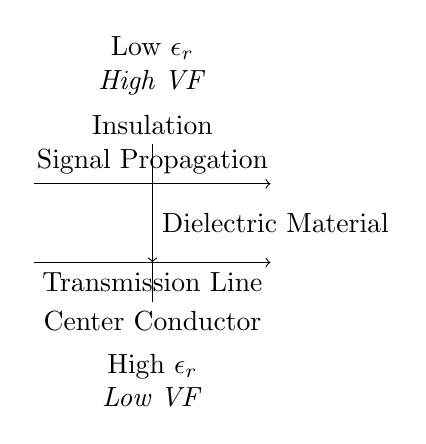
\begin{tikzpicture}
    \draw[->] (0,0) -- (3,0) node[midway, below] {Transmission Line};
    \draw[->] (0,1) -- (3,1) node[midway, above] {Signal Propagation};
    \draw[<-] (1.5,0) -- (1.5,1) node[midway, right] {Dielectric Material};
    \draw (1.5,0) -- (1.5,-0.5) node[below] {Center Conductor};
    \draw (1.5,1) -- (1.5,1.5) node[above] {Insulation};
    
    % Add labels for relative permittivity effect
    \node at (1.5,-1.5) [align=center] {High $\epsilon_r$\\ \textit{Low VF}};
    \node at (1.5,2.5) [align=center] {Low $\epsilon_r$\\ \textit{High VF}};
\end{tikzpicture}

This should provide a clear understanding of how the insulating material of a transmission line affects the velocity factor of signal propagation.